% Two slides: channel persistence 2016-2026, and multiscale (tile) analysis.
% To use in the main deck: copy the two frames below, the figures/ folder,
% and the packages marked "needed by the frames" into the main preamble.
\documentclass[aspectratio=169]{beamer}

% needed by the frames
\usepackage{amsmath}
\graphicspath{{figures/}}

\setbeamertemplate{navigation symbols}{}

\begin{document}

% ---------------------------------------------------------------- slide 1
\begin{frame}{Channel persistence, 2016--2026}
\begin{columns}[T,onlytextwidth]
\begin{column}{0.50\textwidth}
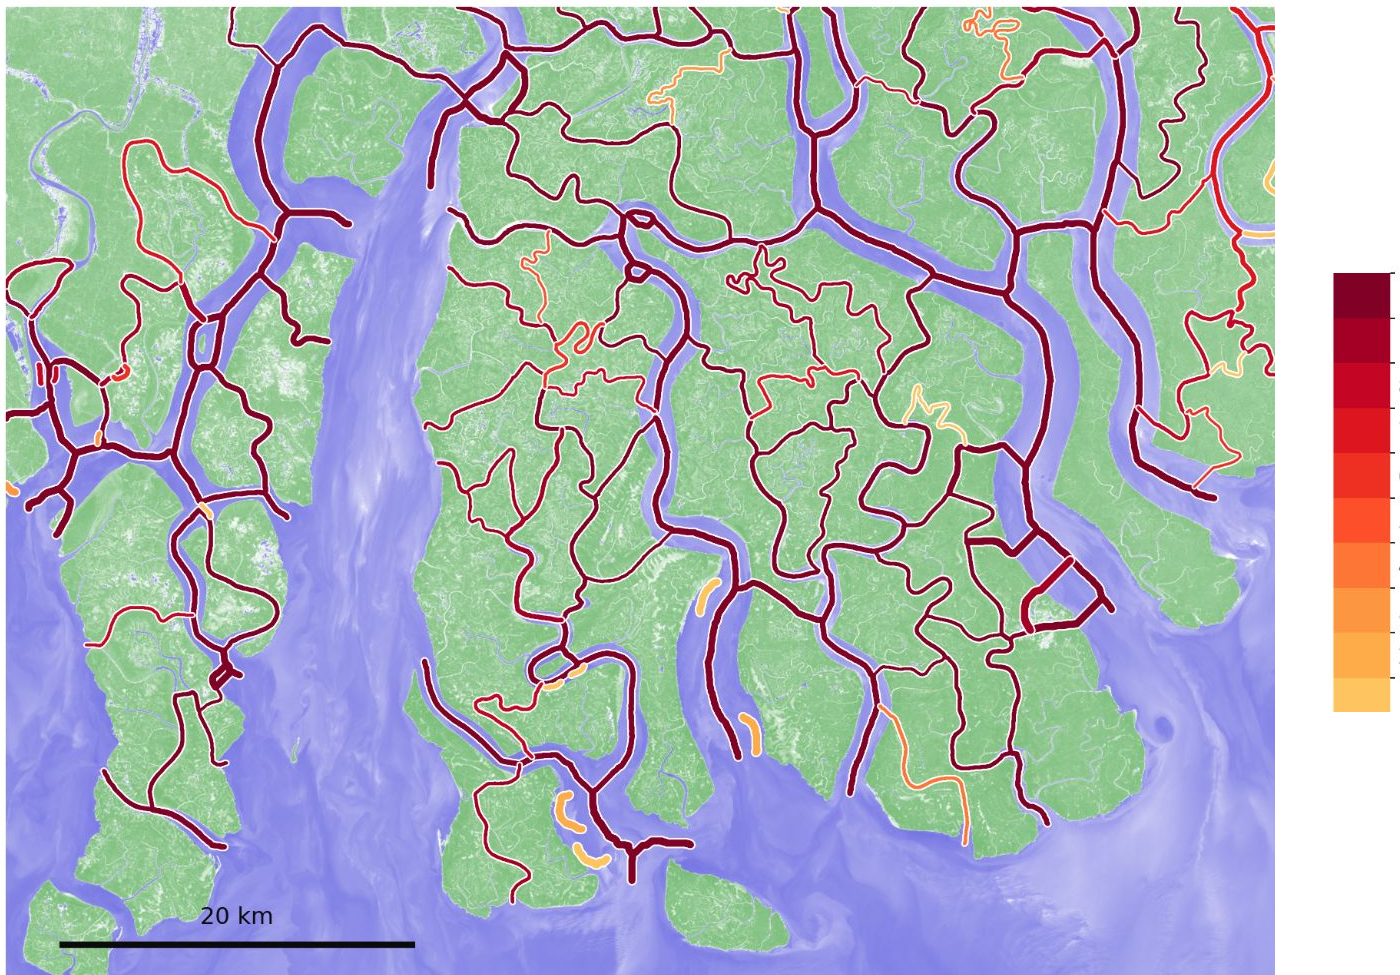
\includegraphics[width=\linewidth]{persistence_map_crop.png}

{\scriptsize Channels on the 2016 image. Colour: number of the 10 snapshots containing the channel (light = 1, dark = 10). Line width = channel width.\par}
\end{column}
\begin{column}{0.48\textwidth}
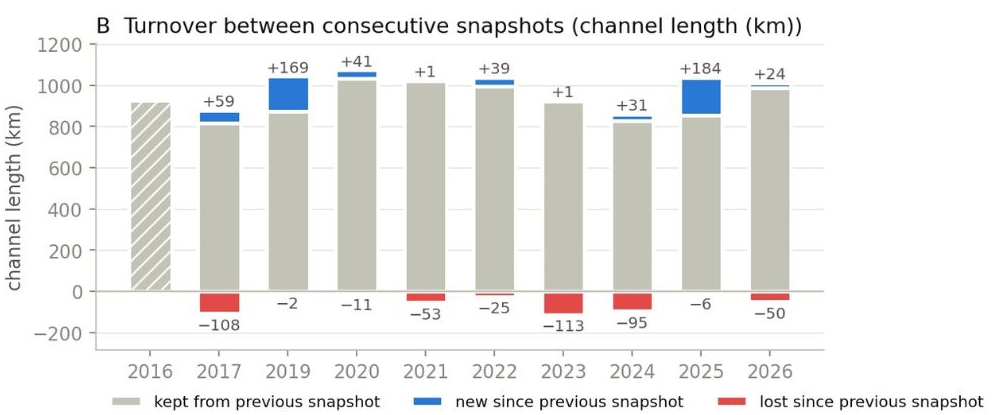
\includegraphics[width=\linewidth]{turnover.png}

\vspace{1mm}
\small
\begin{itemize}\setlength{\itemsep}{3pt}
  \item \alert{66\%} of channel length is in all 10 snapshots (722 of 1,099 km).
  \item Wide main channels persist; changes are in narrow creeks.
  \item Each year gains or loses 0--180 km of about 1,000 km.
  \item Largest losses in 2017, 2023 and 2024; largest gains in 2019 and 2025.
\end{itemize}
\end{column}
\end{columns}
\end{frame}

% ---------------------------------------------------------------- slide 2
\begin{frame}{Multiscale analysis: structure across the delta}
\centering
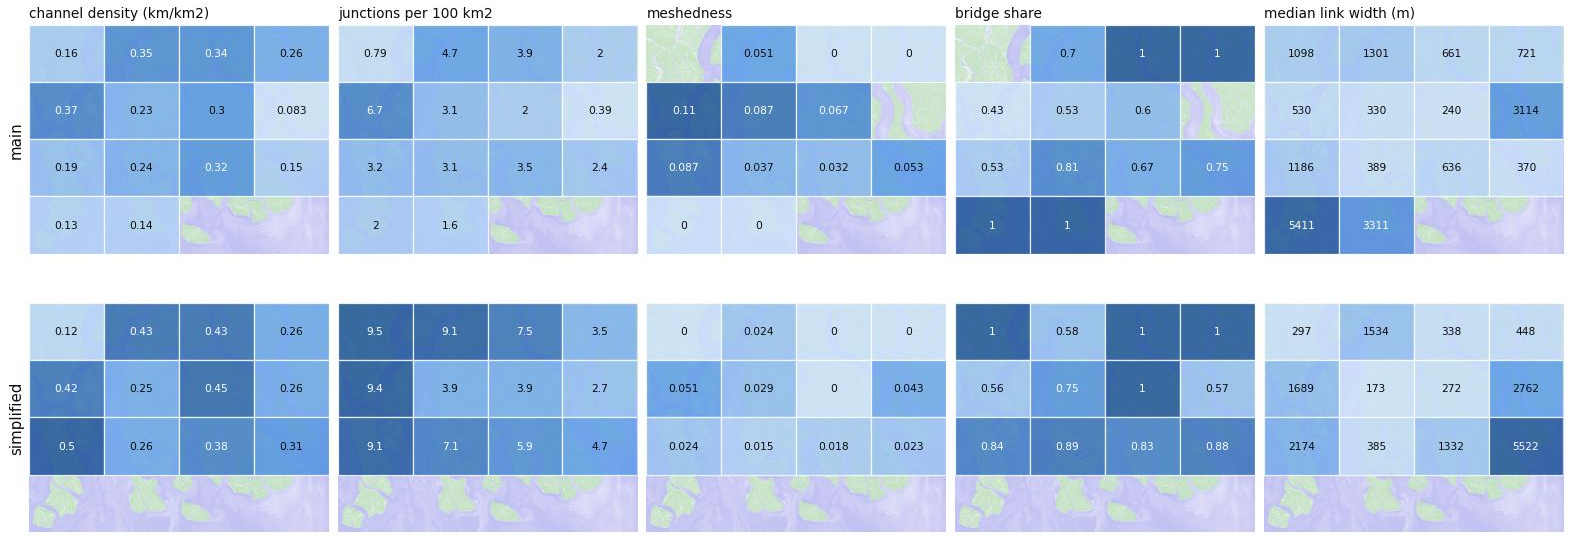
\includegraphics[width=0.96\textwidth]{multiscale.png}

\vspace{1mm}
\raggedright\small
\begin{itemize}\setlength{\itemsep}{1pt}
  \item 4$\times$4 tiles; ratio metrics only for tiles with $\geq$10 nodes; no colour = no usable network.
  \item \textbf{Loops sit inland:} meshedness is highest in the west-central tiles (up to 0.11).
  \item \textbf{The seaward edge is tree-like:} southern tiles have no loops and bridge share 1, along wide estuaries (median width 3--5 km).
  \item Whole-delta averages hide strong local differences.
\end{itemize}
\end{frame}

\end{document}
